\section{Fake Data Appendix}{}
\label{sec:fakedataappendix}

This appendix describes additional studies performed on the fake data.

\subsection{Impact of Optical Filter}

The optical filter was not applied to the fake data.  To investigate the impact of this the muon neutrino selection is plotted both with and without the selection applied in Fig.~\ref{fig:fda:opfilter}. This plot illustrates that the impact of applying the optical filter is within the statistical uncertainty of the selection.

\begin{figure}[H]
\begin{center}
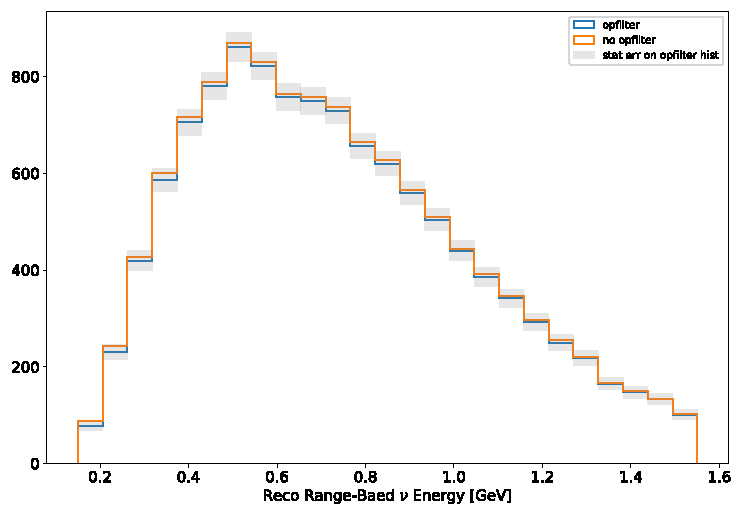
\includegraphics[width=0.45\textwidth]{Fakedata/appendix/opfilter.pdf}
\caption{\label{fig:fda:opfilter} Impact of optical filter on muon neutrino selection.}
\end{center}
\end{figure}

\subsection{Alternate Sensitivity Calculation}
This section describes an alternate sensitivity calculation performed on the fake data.  In this case the sensitivity to rule out the unfolded LEE hypothesis if the standard model is true is calculated. 

Fig.~\ref{fig:fda:altsens_fd1} shows the alternate sensitivity for fake data set 1. The fake data sensitivity to  rule out the standard model if the LEE is true for fake data set 1 is -1.5 $\sigma$. The median sensitivity is 2.1 $\sigma$. 

\begin{figure}[H]
\begin{center}
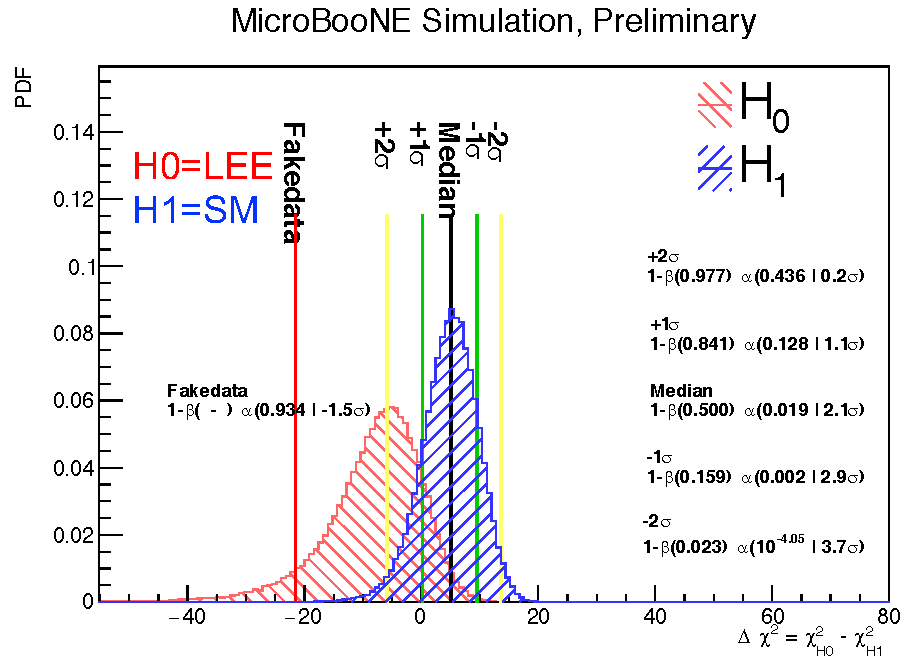
\includegraphics[width=0.45\textwidth]{Fakedata/appendix/altsens_fd1.pdf}
\caption{\label{fig:fda:altsens_fd1} Alternate sensitivity for fake data set 1.}
\end{center}
\end{figure}

Fig.~\ref{fig:fda:altsens_fd2} shows the alternate sensitivity for fake data set 2. The fake data sensitivity to  rule out the standard model if the LEE is true for fake data set 2 is 0.8 $\sigma$. The median sensitivity is 2.5 $\sigma$. 

\begin{figure}[H]
\begin{center}
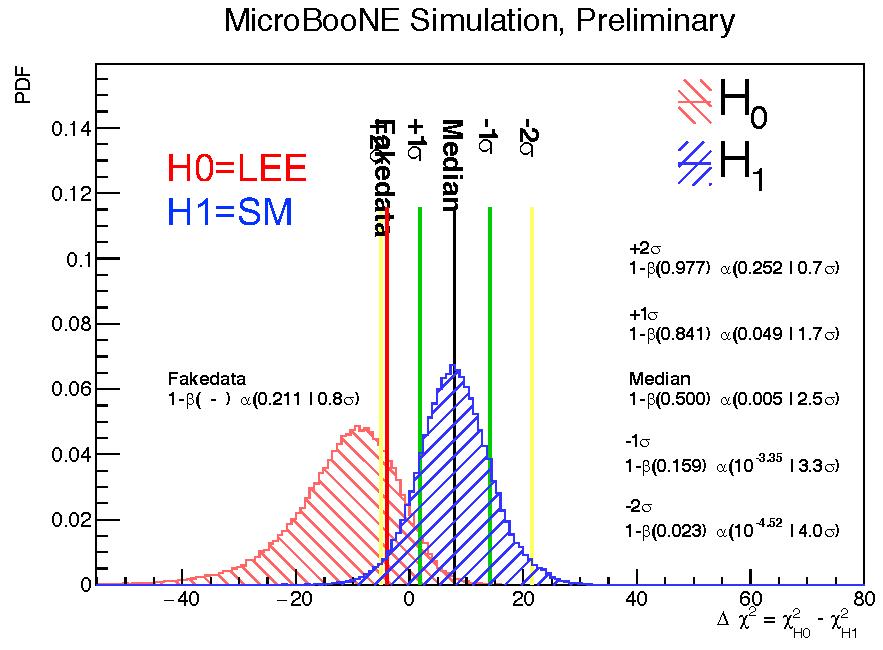
\includegraphics[width=0.45\textwidth]{Fakedata/appendix/altsens_fd2.pdf}
\caption{\label{fig:fda:altsens_fd2} Alternate sensitivity for fake data set 2.}
\end{center}
\end{figure}

Fig.~\ref{fig:fda:altsens_fd3} shows the alternate sensitivity for fake data set 3. The fake data sensitivity to  rule out the standard model if the LEE is true for fake data set 3 is 0.4 $\sigma$. The median sensitivity is 2.5 $\sigma$. 

\begin{figure}[H]
\begin{center}
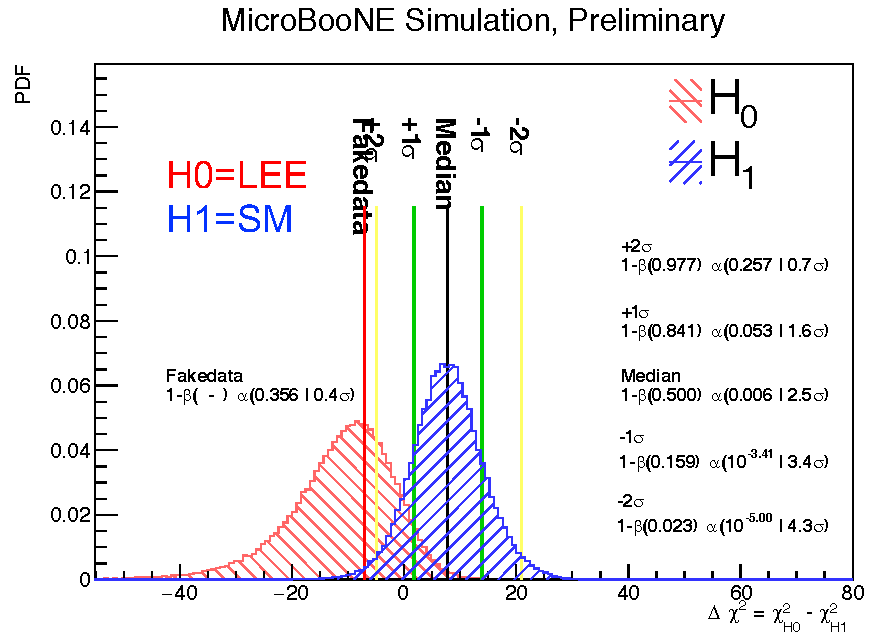
\includegraphics[width=0.45\textwidth]{Fakedata/appendix/altsens_fd3.pdf}
\caption{\label{fig:fda:altsens_fd3} Alternate sensitivity for fake data set 3.}
\end{center}
\end{figure}

The results from this alternate sensitivity study is described in Table~\ref{tab:fakedata:altsens}.

\begin{table}[h!]
\centering
\begin{center}
\begin{tabular}{ c|c|c|c } 
 & Fake Data & Median & Initial Conclusion \\ 
\hline \hline
 Set 1 & -1.5$\sigma$ & 2.1$\sigma$ & \\ 
 Set 2 & 0.8$\sigma$ & 2.5$\sigma$ &  \\ 
 Set 3 & 0.4$\sigma$ & 2.5$\sigma$ &   \\ 
 Set 4 & XX$\sigma$ & YY$\sigma$ &  \\ 
 Set 5 & XX$\sigma$ & YY$\sigma$ &  \\ 
 \hline \hline
\end{tabular}
\end{center}
\caption{Summary of Alternate Sensitivity Fake Data Studies}
\label{tab:fakedata:altsens}
\end{table}

\begin{comment}
\subsection{Impact of First Bin on Sensitivity}

This section describes the impact of removing the lowest energy bin in the sensitivity calculation described in Section~\ref{sec:fakedata}. In this section sensitivity refers to the sensitivity to rule out the standard model if the unfolded LEE model is true.  

Fig.~\ref{fig:fda:nofirstbin_fd1} - Fig.~\ref{fig:fda:nofirstbin_fd3} show the sensitivity with the first bin removed for each of the fake data sets. 

\begin{figure}[H]
\begin{center}
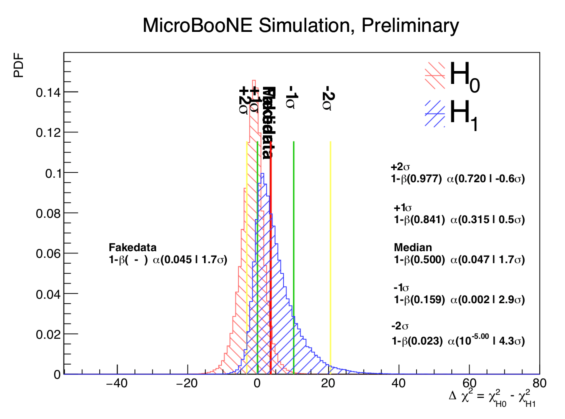
\includegraphics[width=0.45\textwidth]{Fakedata/appendix/nofirstbin_fd1.pdf}
\caption{\label{fig:fda:nofirstbin_fd1} Sensitivity without first bin for fake data set 1.}
\end{center}
\end{figure}

\begin{figure}[H]
\begin{center}
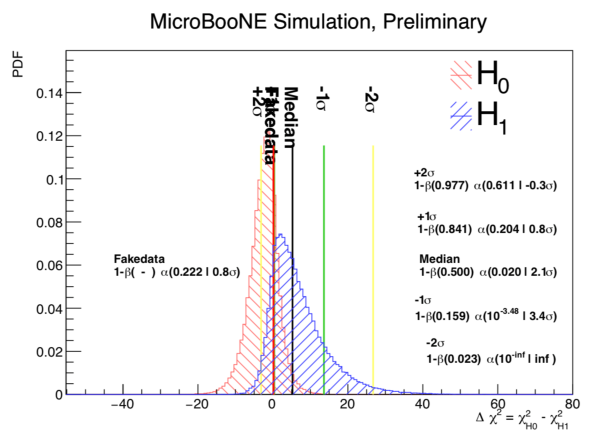
\includegraphics[width=0.45\textwidth]{Fakedata/appendix/nofirstbin_fd2.pdf}
\caption{\label{fig:fda:nofirstbin_fd2} Sensitivity without first bin for fake data set 2.}
\end{center}
\end{figure}

\begin{figure}[H]
\begin{center}
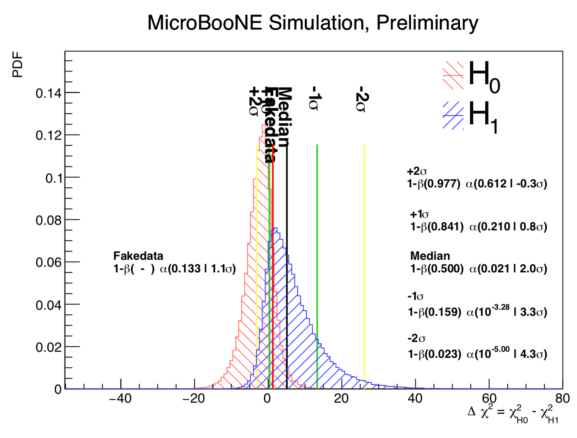
\includegraphics[width=0.45\textwidth]{Fakedata/appendix/nofirstbin_fd3.pdf}
\caption{\label{fig:fda:nofirstbin_fd3} Sensitivity without first bin for fake data set 3.}
\end{center}
\end{figure}

The results from calculating the sensitivity without the lowest energy bin is described in Table~\ref{tab:fakedata:nofirstbin}.  The lowest energy bin can have a large impact on the overall sensitivity.

\begin{table}[h!]
\centering
\begin{center}
\begin{tabular}{ c|c|c|c|c } 
 & Fake Data All Bins & Median All Bins & Fake Data Bin Removed & Median Bin Removed\\ 
\hline \hline
 Set 1 & 3.4$\sigma$ & 2.2$\sigma$& 1.7$\sigma$ & 1.7$\sigma$  \\ 
 Set 2 & 1.9$\sigma$ & 2.6$\sigma$ & 0.8$\sigma$ & 2.1$\sigma$  \\ 
 Set 3 & 2.3$\sigma$ & 2.6$\sigma$& 1.1$\sigma$ & 2.0$\sigma$ \\ 
 Set 4 & XX$\sigma$ & YY$\sigma$ & ZZ$\sigma$& ZZ$\sigma$\\ 
 Set 5 & XX$\sigma$ & YY$\sigma$ & ZZ$\sigma$ & ZZ$\sigma$  \\ 
 \hline \hline
\end{tabular}
\end{center}
\caption{Summary of removing first bin from sensitivity study compared to including it.}
\label{tab:fakedata:nofirstbin}
\end{table}
\end{comment}

\subsection{Sensitivity if Systematic Uncertainties are not Constrained}

The sensitivity was also calculated without including a constraint on the systematic uncertainties. In this section sensitivity refers to the sensitivity to rule out the standard model if the unfolded LEE model is true.  

Fig.~\ref{fig:fda:noconstrain_fd1} - Fig.~\ref{fig:fda:noconstrain_fd3} show the sensitivity with the first bin removed for each of the fake data sets. 

\begin{figure}[H]
\begin{center}
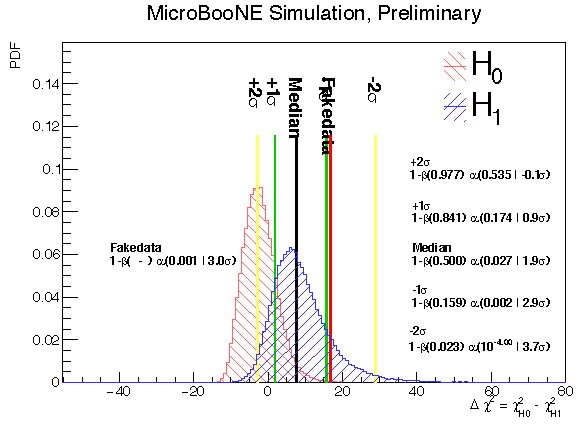
\includegraphics[width=0.45\textwidth]{Fakedata/appendix/noconstrain_fd1.pdf}
\caption{\label{fig:fda:noconstrain_fd1} Sensitivity without constraint of systematic uncertainties for fake data set 1.}
\end{center}
\end{figure}

\begin{figure}[H]
\begin{center}
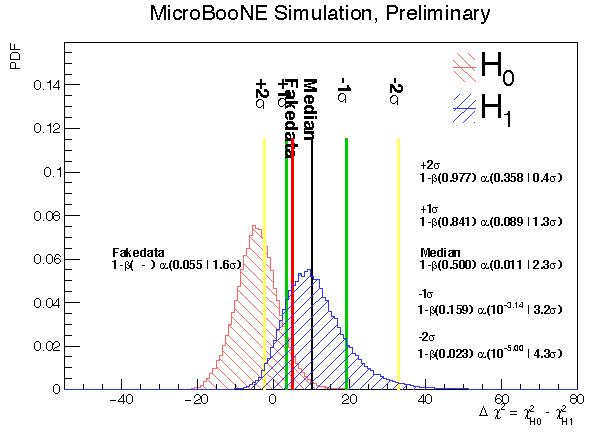
\includegraphics[width=0.45\textwidth]{Fakedata/appendix/noconstrain_fd2.pdf}
\caption{\label{fig:fda:noconstrain_fd2} Sensitivity without constraint of systematic uncertainties for fake data set 2.}
\end{center}
\end{figure}

\begin{figure}[H]
\begin{center}
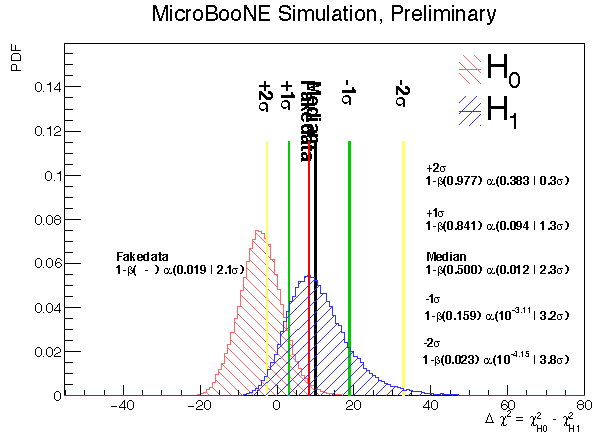
\includegraphics[width=0.45\textwidth]{Fakedata/appendix/noconstrain_fd3.pdf}
\caption{\label{fig:fda:noconstrain_fd3} Sensitivity without constraint of systematic uncertainties for fake data set 3.}
\end{center}
\end{figure}

The results of constraining or not constraining the systematic uncertainties on the sensitivity are shown in Table~\ref{tab:fakedata:noconstrain}.  The median and fake data sensitivity are not as good as with the constraint.

\begin{table}[h!]
\centering
\begin{center}
\begin{tabular}{ c|c|c|c|c } 
 & Fake Data All Bins & Median All Bins & Fake Data Bin Removed & Median Bin Removed\\ 
\hline \hline
 Set 1 & 3.4$\sigma$ & 2.2$\sigma$& 3.0$\sigma$ & 1.9$\sigma$  \\ 
 Set 2 & 1.9$\sigma$ & 2.6$\sigma$ & 1.6$\sigma$ & 2.3$\sigma$  \\ 
 Set 3 & 2.3$\sigma$ & 2.6$\sigma$& 2.1$\sigma$ & 2.3$\sigma$ \\ 
 Set 4 & XX$\sigma$ & YY$\sigma$ & ZZ$\sigma$& ZZ$\sigma$\\ 
 Set 5 & XX$\sigma$ & YY$\sigma$ & ZZ$\sigma$ & ZZ$\sigma$  \\ 
 \hline \hline
\end{tabular}
\end{center}
\caption{Impact of constraining systematic uncertainties on the sensitivity.}
\label{tab:fakedata:noconstrain}
\end{table}